\documentclass[12pt]{article}
\usepackage{fullpage,enumitem,amsmath,amssymb,graphicx}

\title{College Physics Homework 1 }
%\author{Deniz O. Devecioglu  -- \texttt{dodeve@gmail.com}}

\begin{document}
  \maketitle,
  \begin{center}

  \vspace{-0.3in}
  \begin{tabular}{rl}
  Due: March 18 2022 & 
  \end{tabular}
  \end{center}
  This is an individual assignment; you must solve it by yourself.
  \noindent

  \rule{\linewidth}{0.4pt}
\section*{Problem 1}
A vector has components $A_x=5.0$, $A_{y}=-3.0$, $A_{z}=1.0$. What is the magnitude of this vector? What is the angle between this vector and the $x$ axis? The $y$ axis? The $z$ axis?

  \section*{Problem 2}
The refraction of light can be understood by purely kinematical considerations. We need to assume that light takes the shortest (timewise) path between two points (Fermat's principle of least time.) Referring to the Fig \ref{fig1}, let the speed of light in medium 1 be $v_{1}$ and in medium 2, $v_{2}$. Calculate the time it takes light to go from point $A$ to point $B$ as a function of variable $x$. Minimize with respect to $x$. 
\newline 
Given that
\begin{align}
v_{1}=c/n_{1},\quad and \quad v_{2}=c/n_{2}
\end{align}
where $n$'s are known as indices of refraction, prove Snell's law of refraction.
\begin{align}
n_{1}\sin\theta_{1}=n_{2}\sin\theta_{2}.
\end{align}
\begin{figure}
\center
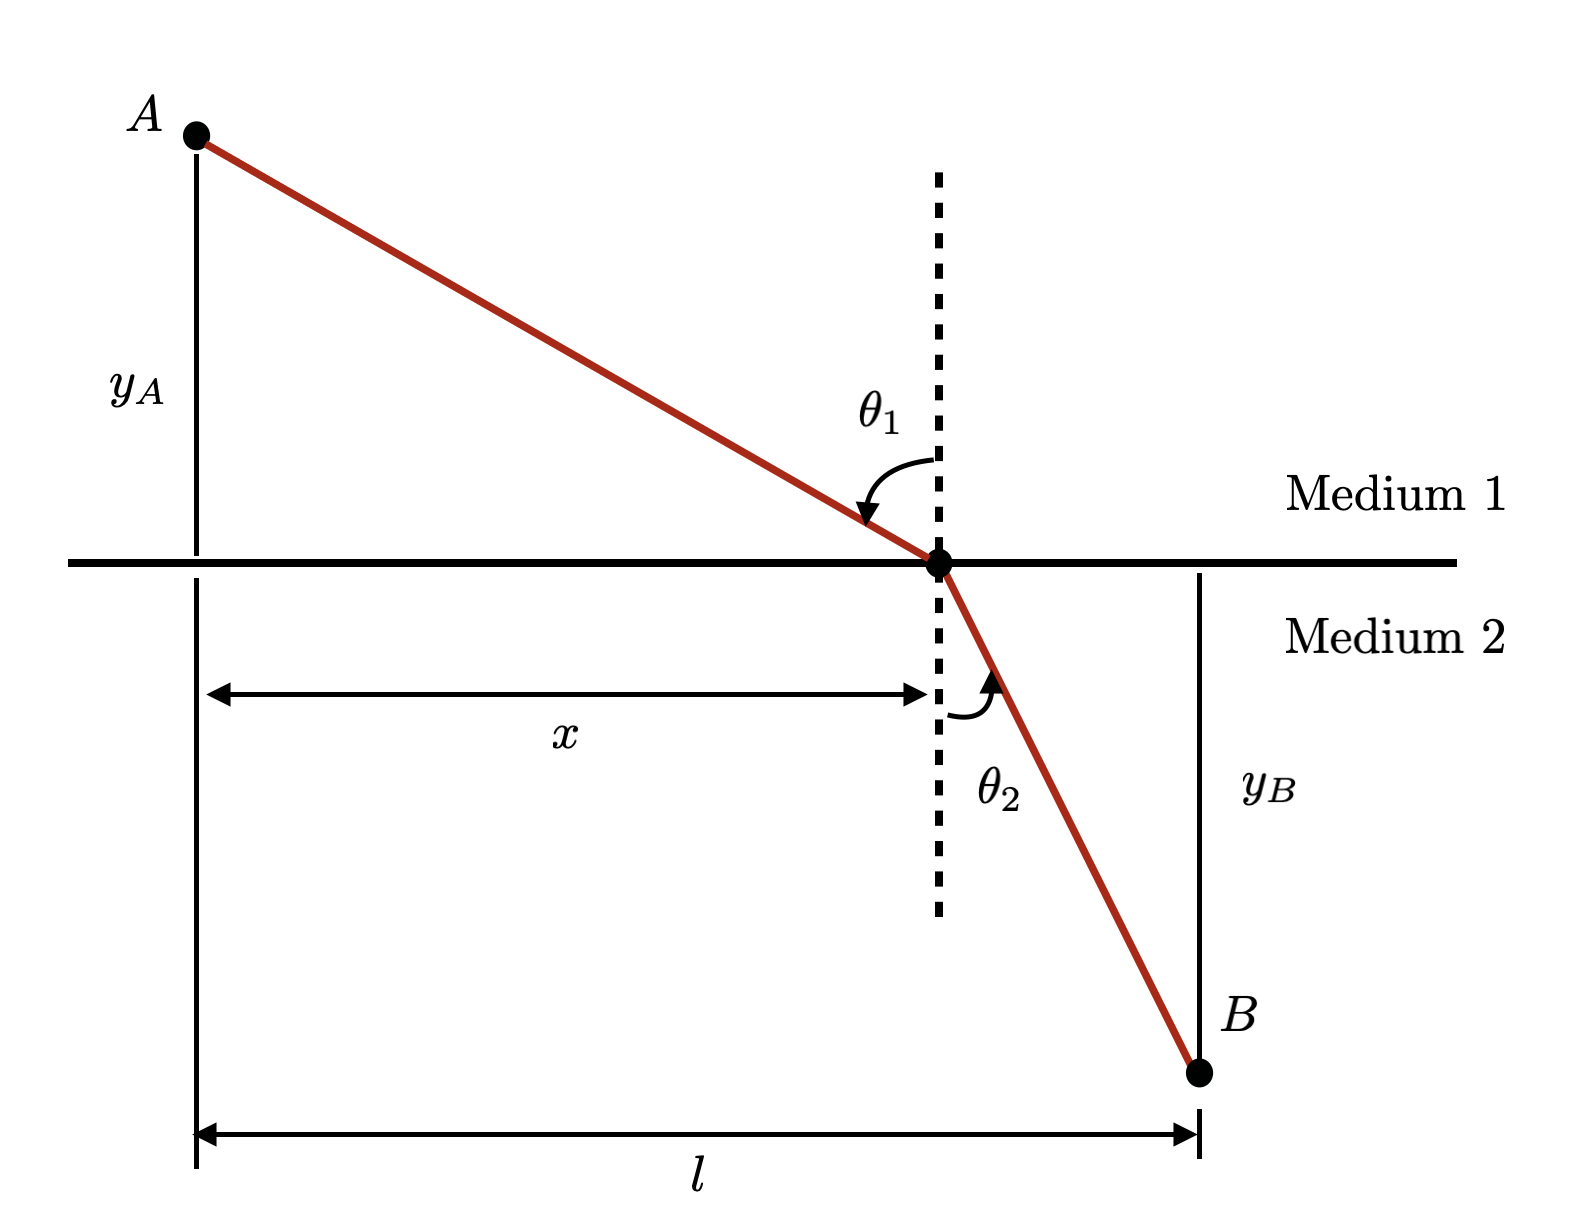
\includegraphics[scale=0.4]{refraction}
\caption{Figure for problem 2}\label{fig1}
\end{figure}
\newpage
  \section*{Problem 3}
Suppose you throw a stone straight up with an initial speed of $15.0$ m/s.
\begin{enumerate}[label=$\roman*$)]
\item If you throw a second stone straight up $1.00$s after the first, with what speed must you throw the second stone if it is to hit the first at a height of $11.0 $m? (There are two answers. Are both plausible?)
\item If you throw the second stone $1.30$ s after the first, with what speed must you throw the second stone if it is to hit the first at a height of $11.0$ m?
\end{enumerate}

  \section*{Problem 4}
A perfectly elastic ball is thrown to a wall and bounces back over the head of the thrower (Fig \ref{fig2}). It is thrown height $a$ above the ground and distance $c$ from the wall, and has $v_{0x}=v_{0y}=v$. How far behind the thrower does the ball hit the ground ?
\begin{figure}
\center
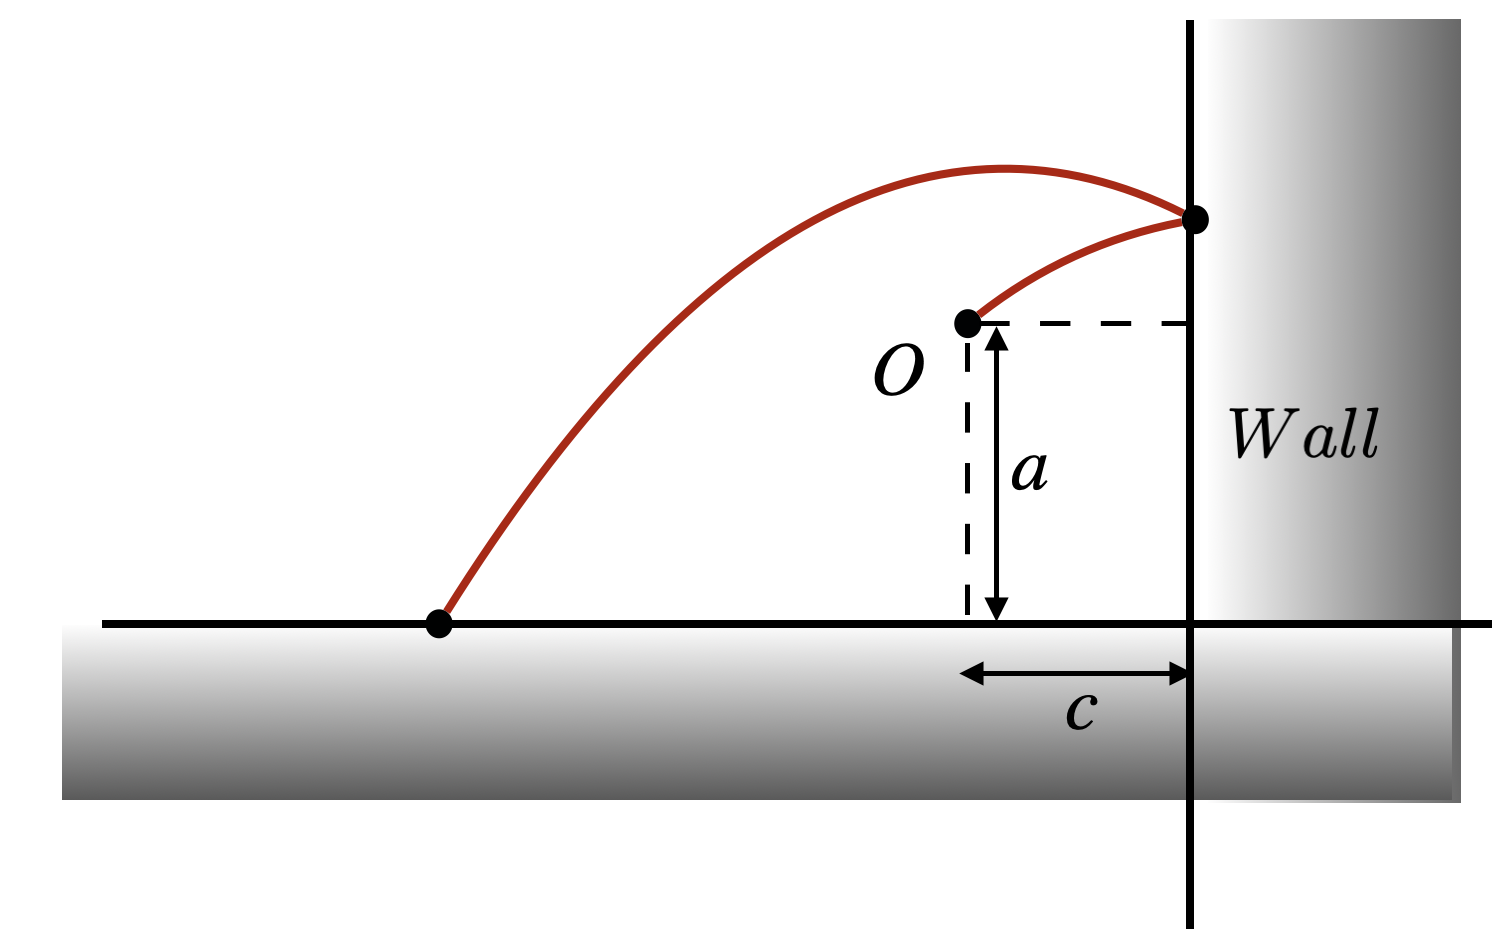
\includegraphics[scale=0.4]{projectile}
\caption{Projectile motion for problem 4}\label{fig2}
\end{figure}
 \section*{Problem 5}
An airplane, whose air speed is $580$ km/h is supposed to fly in a straight path $38$ North of East. But steady $72$ km/h wind is blowing from the north. In what direction should the plane head?
\end{document}



